% \begin{figure*}
% \centering
% \begin{minipage}{.5\textwidth}
%     \includegraphics[width=\linewidth]{durationDiagramCPU.pdf}
%     \captionof{figure}{CPU: Average facial expression calculation wall time}
%     \label{fig:RuntimeCost}
% \end{minipage}%
% \hfill
% \begin{minipage}{.5\textwidth}
%     \includegraphics[width=\linewidth]{durationDiagramCUDA.pdf}
%     \captionof{figure}{GPU: Average wall time for 10 concurrent facial expression calculations}
%     \label{fig:RuntimeCostGPU}
% \end{minipage}
% \hfill
% \begin{minipage}{.33\textwidth}
%     \includegraphics[width=\linewidth]{compressionRatesDiagram.pdf}
%     \captionof{figure}{Compression Rates relative to sparse blendshapes size}
%     \label{fig:Compression}
% \end{minipage}
% \end{figure*}

\begin{figure*}[p]
  \subfloat[Aura]{\includegraphics[width=0.29\linewidth]{modelAura.png}} \hspace{.5cm}
  \subfloat[Bowen]{\includegraphics[width=0.29\linewidth]{modelBoz.png}} \hspace{.5cm}
  \subfloat[Jupiter]{\includegraphics[width=0.29\linewidth]{modelJupiter.png}} \\
   % \vspace{1em}
  \subfloat[Proteus]{\includegraphics[width=0.29\linewidth]{modelProteus.png}}\hspace{.5cm}
  \subfloat[Louise]{\includegraphics[width=0.29\linewidth]{modelLouise.png}}\hspace{.5cm}
  \subfloat[Carlos]{\includegraphics[width=0.29\linewidth]{modelCarlos.png}}
    % \vspace{1em}
\caption{Images rendered from the datasets used for experiments.}
\label{fig:Datasets}
\end{figure*}


% \begin{figure*}
%   \includegraphics[width=0.6\linewidth]{durationDiagramCPU.pdf}
%   \vspace{-.33em}
%     \captionof{figure}{CPU: Average facial expression calculation wall time}
% \vspace{-.55em}
%     \label{fig:RuntimeCost}
%   \end{figure*}
% \begin{figure*}
%   \includegraphics[width=0.6\linewidth]{durationDiagramCUDA.pdf}
%   \vspace{-.33em}
%     \captionof{figure}{GPU: Average wall time for 10 concurrent facial expression calculations}
%  \vspace{-.55em}
%    \label{fig:RuntimeCostGPU}
% \end{figure*}
% \begin{figure*}
% \includegraphics[width=0.6\linewidth]{compressionRatesDiagram.pdf}
%      \vspace{-.33em}
%      \captionof{figure}{Compression Rates relative to sparse blendshapes size}
%      \vspace{-.55em}
%     \label{fig:Compression}
% \end{figure*}
%
%
% \begin{figure*}[p]
%   \subfloat[Aura]{\includegraphics[width=0.3\linewidth]{modelAura.png}} \hspace{1em}
%   \subfloat[Bowen]{\includegraphics[width=0.3\linewidth]{modelBoz.png}} \hspace{1em}
%   \subfloat[Jupiter]{\includegraphics[width=0.3\linewidth]{modelJupiter.png}} \\
%    % \vspace{1em}
%   \subfloat[Proteus]{\includegraphics[width=0.3\linewidth]{modelProteus.png}}\hspace{1em}
%   \subfloat[Louise]{\includegraphics[width=0.3\linewidth]{modelLouise.png}}\hspace{1em}
%   \subfloat[Carlos]{\includegraphics[width=0.3\linewidth]{modelCarlos.png}}
%     % \vspace{1em}
% \caption{Images rendered from the datasets used for experiments.}
% \label{fig:Datasets}
% \end{figure*}

%-----
% \newcommand{\lineOfImages}[2]{
% \rotatebox[origin=c]{90}{\centering #2} &
% \raisebox{-.5\height}{\includegraphics[width=0.15\linewidth, trim=0pt -1mm 0pt -1mm]{#1NoseOrig.png}\ifthenelse{\equal{#1}{proteus}}{\llap{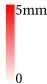
\includegraphics[height=0.075\linewidth]{legendDistanceMap.pdf}}}{}
% }&
% \raisebox{-.5\height}{\includegraphics[width=0.15\linewidth, trim=0pt -1mm 0pt -1mm]{#1NoseCSFB.png}} &
% \raisebox{-.5\height}{\includegraphics[width=0.15\linewidth, trim=0pt -1mm 0pt -1mm]{#1NoseQMF.png}} &
% \raisebox{-.5\height}{\includegraphics[width=0.15\linewidth, trim=0pt -1mm 0pt -1mm]{#1ForeheadOrig.png}} &
% \raisebox{-.5\height}{\includegraphics[width=0.15\linewidth, trim=0pt -1mm 0pt -1mm]{#1ForeheadCSFB.png}} &
% \raisebox{-.5\height}{\includegraphics[width=0.15\linewidth, trim=0pt -1mm 0pt -1mm]{#1ForeheadQMF.png}}
% }
% \begin{figure*}[p]
%     \setlength{\tabcolsep}{2pt}
%     % \renewcommand{\arraystretch}{9}
%     \begin{tabular}{c c c c c c c}
%       % \hline
%       \lineOfImages{aura}{Aura} \\
%       \lineOfImages{bowen}{Bowen} \\
%       \lineOfImages{jupiter}{Jupiter}  \\
%     \lineOfImages{proteus}{Proteus} \\
%       &Original & CSFB& QMF& Original & CSFB& QMF \\
%     \end{tabular}
%     \caption{\add{A visual inspection of error of CSFB vs QMF.  The error visualized in red is the vertex distance between uncompressed and the CSFB and QMF compressed methods.}}
% \label{fig:poses}
% \end{figure*}

%--------------------------------------exp---------------------------------------

% \begin{minipage}[b]{35mm}
%   \includegraphics[width=35mm]{auraNoseOrig.png}
% \end{minipage}



\newcommand{\poseWidth}{28mm}
\newcommand{\onePose}{
}
\newcommand{\lineOfImagesNoTable}[2]{
\rotatebox[origin=c]{90}{\centering #2}
% \raisebox{-.5\height}{\includegraphics[width=\poseWidth]{#1NoseOrig.png}\llap{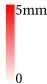
\includegraphics[height=0.075\linewidth]{legendDistanceMap.pdf}}}
\raisebox{-.5\height}{\includegraphics[width=\poseWidth]{#1NoseOrig.png}\llap{\ifthenelse{\equal{#1}{proteus}}{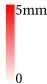
\includegraphics[height=0.090\linewidth]{legendDistanceMap.pdf}}{}}}
\raisebox{-.5\height}{\includegraphics[width=\poseWidth]{#1NoseCSFB.png}}
\raisebox{-.5\height}{\includegraphics[width=\poseWidth]{#1NoseQMF.png}}
\raisebox{-.5\height}{\includegraphics[width=\poseWidth]{#1ForeheadOrig.png}}
\raisebox{-.5\height}{\includegraphics[width=\poseWidth]{#1ForeheadCSFB.png}}
\raisebox{-.5\height}{\includegraphics[width=\poseWidth]{#1ForeheadQMF.png}} 
\vspace{1mm}
}
\newcommand{\lineOfCaptions}{
  \rotatebox[origin=c]{90}{\centering \phantom{c} }
\begin{minipage}[c]{28mm}
 \centering Original
\end{minipage}
\begin{minipage}[c]{28mm}
 \centering CSFB
\end{minipage}
\begin{minipage}[c]{28mm}
 \centering QMF
\end{minipage}
\begin{minipage}[c]{28mm}
 \centering Original
\end{minipage}
\begin{minipage}[c]{28mm}
 \centering CSFB
\end{minipage}
\begin{minipage}[c]{28mm}
 \centering QMF
\end{minipage}
}

\begin{figure*}[p]
  \lineOfImagesNoTable{aura}{Aura} \\
  \lineOfImagesNoTable{bowen}{Bowen} \\
  \lineOfImagesNoTable{jupiter}{Jupiter} \\
  \lineOfImagesNoTable{proteus}{Proteus} \\
  \lineOfCaptions
    \caption{\add{A visual inspection of error of CSFB vs QMF.  The error visualized in red is the vertex distance between uncompressed and the CSFB and QMF compressed methods.}}
\label{fig:poses}
\end{figure*}
